\documentclass[ignorenonframetext,11pt,xcolor=dvipsnames,aspectratio=1610,hyperref={bookmarksdepth=4}]{beamer}
\setbeamertemplate{caption}[numbered]
\setbeamertemplate{caption label separator}{: }
\setbeamercolor{caption name}{fg=normal text.fg}
\beamertemplatenavigationsymbolsempty
\usepackage{lmodern}
\usepackage{amssymb,amsmath}
\usepackage{ifxetex,ifluatex}
\usepackage{fixltx2e} % provides \textsubscript
\ifnum 0\ifxetex 1\fi\ifluatex 1\fi=0 % if pdftex
  \usepackage[T1]{fontenc}
  \usepackage[utf8]{inputenc}
\else % if luatex or xelatex
  \ifxetex
    \usepackage{mathspec}
  \else
    \usepackage{fontspec}
  \fi
  \defaultfontfeatures{Ligatures=TeX,Scale=MatchLowercase}
\fi
% use upquote if available, for straight quotes in verbatim environments
\IfFileExists{upquote.sty}{\usepackage{upquote}}{}
% use microtype if available
\IfFileExists{microtype.sty}{%
\usepackage{microtype}
\UseMicrotypeSet[protrusion]{basicmath} % disable protrusion for tt fonts
}{}
\newif\ifbibliography
\hypersetup{
            pdftitle={广义可加混合模型基于切片抽样MCMC估计与PQL估计比较研究},
            pdfauthor={李研},
            pdfborder={0 0 0},
            breaklinks=true}
\urlstyle{same}  % don't use monospace font for urls

% Prevent slide breaks in the middle of a paragraph:
\widowpenalties 1 10000
\raggedbottom

\AtBeginPart{
  \let\insertpartnumber\relax
  \let\partname\relax
  \frame{\partpage}
}
\AtBeginSection{
  \ifbibliography
  \else
    \let\insertsectionnumber\relax
    \let\sectionname\relax
    \frame{\sectionpage}
  \fi
}
\AtBeginSubsection{
  \let\insertsubsectionnumber\relax
  \let\subsectionname\relax
  \frame{\subsectionpage}
}

\setlength{\parindent}{0pt}
\setlength{\parskip}{6pt plus 2pt minus 1pt}
\setlength{\emergencystretch}{3em}  % prevent overfull lines
\providecommand{\tightlist}{%
  \setlength{\itemsep}{0pt}\setlength{\parskip}{0pt}}
\setcounter{secnumdepth}{0}

\author{李研}

\date{\today}
\date{2019-05}

\usepackage[BoldFont,SlantFont]{xeCJK}
\setCJKmainfont[BoldFont=Microsoft YaHei]{SimSun}

\usepackage[BoldFont,SlantFont]{xeCJK}

\setCJKmainfont[BoldFont=AdobeHeitiStd-Regular]{AdobeSongStd-Light}
\setCJKfamilyfont{song}{AdobeSongStd-Light}
\setCJKfamilyfont{hei}{AdobeHeitiStd-Regular}
\setCJKfamilyfont{kai}{AdobeKaitiStd-Regular}
\setCJKfamilyfont{fs}{Sun Yat-sen Hsingshu}

\author[李\; 研(中南财经政法大学统计与数学学院)]{\CJKfamily{kai} 李 \enspace 研 \\ 中南财经政法大学统计与数学学院 \\ 经济统计学}



\renewcommand{\contentsname}{\centerline{\textcolor{violet}{目 \ \ 录}}}    % 将Contents改为目录
\renewcommand{\abstractname}{摘 \ \ 要}      % 将Abstract改为摘要
\renewcommand{\refname}{参考文献}            % 将Reference改为参考文献
\renewcommand\tablename{表}
\renewcommand\figurename{图}
\renewcommand{\today}{\number\year 年 \number\month 月 \number\day 日}

\PassOptionsToPackage{dvipsnames}{xcolor}
\PassOptionsToPackage{colorlinks=true,citecolor=blue, urlcolor=blue, linkcolor=violet, bookmarksdepth=4}{hyperref}

\usepackage{lscape}
\usepackage{indentfirst}
\usepackage{textcomp}                      % provide many text symbols
\usepackage{setspace}                      % 各种间距设置


% ---------------------------------Table------------------------------
\usepackage{booktabs}
\usepackage{array}                         % 提供表格中每一列的宽度及位置支持
\usepackage{multirow}
\usepackage{rotating}
\newcolumntype{L}[1]{>{\raggedright\let\newline\\\arraybackslash\hspace{0pt}}m{#1}}
\newcolumntype{C}[1]{>{\centering\let\newline\\\arraybackslash\hspace{0pt}}m{#1}}
\newcolumntype{R}[1]{>{\raggedleft\let\newline\\\arraybackslash\hspace{0pt}}m{#1}}

%\sloppy
%\linespread{1.0}                           % 设置行距
\setlength{\parindent}{18pt}
%\setlength{\parskip}{1ex plus 0.5ex minus 0.2ex}


\usepackage[utf8]{inputenc}
% Package fontenc omitted
% Package fixltx2e omitted
\usepackage{graphicx}
% Package longtable omitted
% Package float omitted
% Package wrapfig omitted
\usepackage{soul}
% Package textcomp omitted
\usepackage{marvosym}
\usepackage{wasysym}
\usepackage{latexsym}
\usepackage{amssymb}
\usepackage{lmodern,bm}
% Package hyperref omitted
\usepackage{listings}
\usepackage{tikz}

						   
\setmonofont{Consolas} % listings 中支持 consolas 字体,必需配合上面usepackage{fontenc} 中不出现[T1]才可以

\lstset{numbers=left, numberstyle=\ttfamily\tiny\color{Gray}, stepnumber=1, numbersep=8pt,
  frame=leftline,
  framexleftmargin=0mm,
  rulecolor=\color{CadetBlue},
  backgroundcolor=\color{Periwinkle!20},
  stringstyle=\color{CadetBlue},
  flexiblecolumns=false,
  aboveskip=5pt,
  belowskip=0pt,
  language=R,
  basicstyle=\ttfamily\footnotesize,
  columns=flexible,
  keepspaces=true,
  breaklines=true,
  extendedchars=true,
  texcl=false,  % 必须设置为false设置为true的时候 R 代码中不能含有多个注释符号 #
  upquote=true, % 设置 引号为竖引号,但必需配合 上面 fontenc T1 使用,fontenc T1 又不能使用 consolas,所以冲突
  showstringspaces=false,
  keywordstyle=\bfseries,
  keywordstyle=\color{Purple},
  xleftmargin=20pt,
  xrightmargin=10pt,
  morecomment=[s]{\#}{\#},
  commentstyle=\color{OliveGreen!60}\scriptsize,
  tabsize=4}

\tolerance=1000
\usetheme{default}
\setcounter{secnumdepth}{4}

\usetheme{default}
\useinnertheme[shadow]{rounded}
\useoutertheme{infolines}
\usecolortheme{seahorse}
\setbeamercolor{frametitle}{fg=Blue, bg=white}
\setbeamercolor{titlelike}{parent=structure}
\setbeamertemplate{caption}[numbered]
\setbeamertemplate{section in toc shaded}[default][50]
\setbeamertemplate{frametitle continuation}[from second][(续)] % 改变
\setbeamertemplate{subsection in toc shaded}[default][20]
\setbeamertemplate{subsection in toc}[square]
\logo{
\includegraphics[height=0.6cm,width=0.6cm]{znufelogo.jpg}}
\setbeamercovered{transparent}
\setCJKmainfont[BoldFont={* Bold}]{Microsoft YaHei}
\usefonttheme[onlylarge]{structuresmallcapsserif}
\usefonttheme[onlymath]{serif}
\setbeamertemplate{frametitle}{\bfseries\insertframetitle\par\vskip-6pt}
\AtBeginSection[]
{
\setcounter{tocdepth}{2}
\frame[shrink=5]{\tableofcontents[currentsection, hideothersubsections]}
}
\AtBeginSubsection[] % Do nothing for \subsection*
{
\begin{frame}<beamer>
\frametitle{}
\Large \tableofcontents[currentsubsection,sectionstyle=hide/hide, subsectionstyle=show/shaded/hide]
\end{frame}
}
\setlength{\parskip}{1ex plus 0.5ex minus 0.2ex}
\everydisplay{\color{blue}}


\title{广义可加混合模型基于切片抽样MCMC估计与PQL估计比较研究}


\begin{document}
\frame{\titlepage}

\section{选题背景及意义}

\begin{frame}{选题背景}

(1)广义可加混合模型既考虑了协变量的线性影响,又考虑了非线性影响,同时考虑了随机
效应,在实际问题分析中,模型设定可能更为精确。

(2)GAMM的推断基于似然原理,会涉及高维积分的计算。惩罚拟似然(PQL)是经常采用的
一种估计方法,但在使用中逐渐暴露出一些问题。相应的,基于马尔可夫链蒙特卡罗(MCMC)
的贝叶斯估计备受关注。在MCMC的抽样方法中,Neal(2003)提出切片抽样比Gibbs采样实施
起来更加简单,比M-H抽样更加有效。

(3)为证明GAMM的实用性,考虑GAMM在空气质量方面的应用。近年来,空气质量问题引起了社会
各界的广泛关注,中国粗放型的经济发展模式使空气质量在逐年恶化,空气质量状况的日益下降
警醒我们须及时采取环境保护的相关措施。这就需要我们找到空气质量的影响因素,进而根据影响
因素及影响程度的大小进行相应的处理。

\end{frame}

\begin{frame}{选题意义}

(1)理论意义

用基于切片抽样的MCMC方法与PQL方法进行估计精度的比较,可以验证GAMM更加精确的参数估计
方法,为用GAMM进行数据分析提供参考。

(2)现实意义

一方面,以74个城市月度数据建立GAMM进行分析,选择精度较高的估计方法对所建立的模型进行
估计,可以对空气质量做出更加精确的预测,进而为环境治理决策提供更加有效的支撑。

另一方面,目前,空气污染非常严重,研究城市空气质量的影响因素,可以证明针对中国的实际
情况,气象因素和经济因素对空气质量的具体影响效应,及时对短期内空气质量情况进行较为
准确的简单预报,对空气质量的改善有极大的推动作用。

\end{frame}

\section{主要内容、基本思路及论文提纲}

\begin{frame}{主要内容}

第一部分、第二部分:

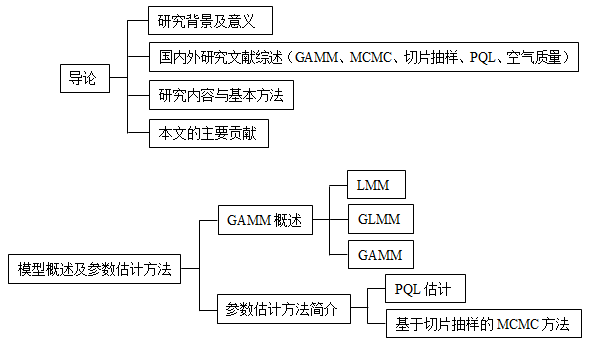
\includegraphics[width=8.39in]{2}

\end{frame}

\begin{frame}{主要内容(续)}

第三部分:

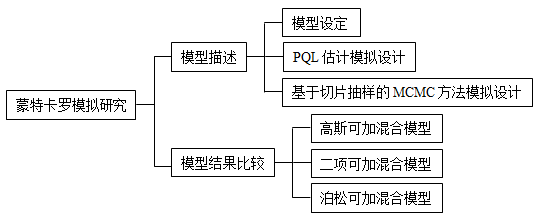
\includegraphics[width=7.51in]{3}

\end{frame}

\begin{frame}{主要内容(续)}

第四部分:

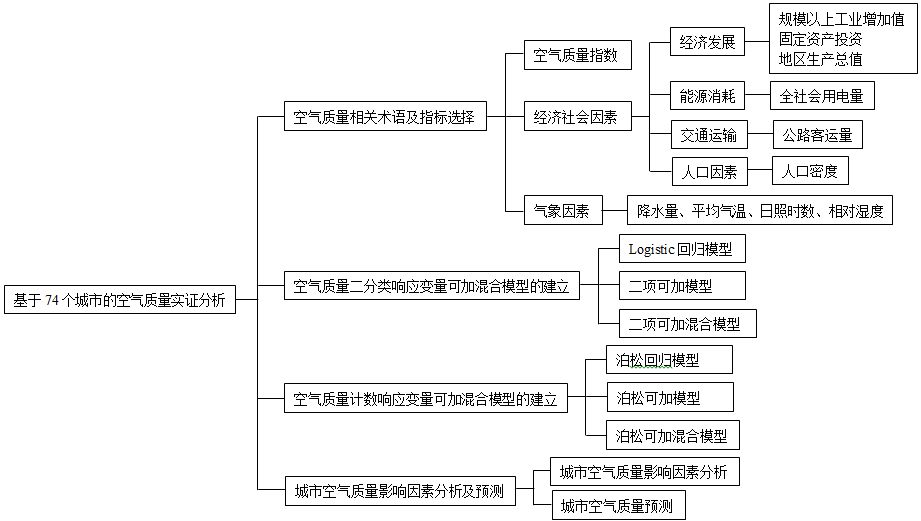
\includegraphics[width=12.79in]{4}

\end{frame}

\begin{frame}{主要内容(续)}

第五部分:

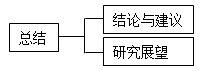
\includegraphics[width=2.82in]{5}

\end{frame}

\begin{frame}{基本思路}

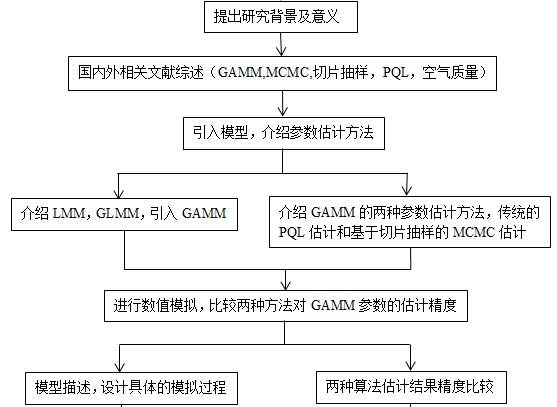
\includegraphics[width=7.74in]{6_1}

\end{frame}

\begin{frame}{基本思路(续)}

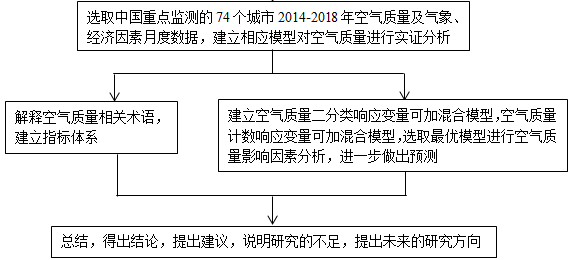
\includegraphics[width=7.9in]{6_2}

\end{frame}

\begin{frame}{论文提纲}

\begin{itemize}
\tightlist
\item
  导论

  \begin{itemize}
  \tightlist
  \item
    一、研究背景及意义
  \item
    二、国内外研究文献综述
  \item
    三、研究内容与基本方法
  \item
    四、本文的主要贡献
  \end{itemize}
\item
  第一章 模型概述及参数估计方法

  \begin{itemize}
  \tightlist
  \item
    第一节 GAMM概述

    \begin{itemize}
    \tightlist
    \item
      一、线性混合模型(LMM)
    \item
      二、广义线性混合模型(GLMM)
    \item
      三、广义可加混合模型(GAMM)
    \end{itemize}
  \item
    第二节 参数估计方法简介

    \begin{itemize}
    \tightlist
    \item
      一、惩罚拟似然估计(PQL)
    \item
      二、基于切片抽样的MCMC方法
    \end{itemize}
  \end{itemize}
\end{itemize}

\end{frame}

\begin{frame}{论文提纲(续)}

\begin{itemize}
\tightlist
\item
  第二章 蒙特卡罗模拟研究

  \begin{itemize}
  \tightlist
  \item
    第一节 模型描述

    \begin{itemize}
    \tightlist
    \item
      一、模型设定
    \item
      二、惩罚拟似然估计模拟设计
    \item
      三、基于切片抽样的MCMC估计模拟设计
    \end{itemize}
  \item
    第二节 模拟结果比较

    \begin{itemize}
    \tightlist
    \item
      一、高斯可加混合模型下模拟结果比较
    \item
      二、二项可加混合模型下模拟结果比较
    \item
      三、泊松可加混合模型下模拟结果比较
    \end{itemize}
  \end{itemize}
\end{itemize}

\end{frame}

\begin{frame}{论文提纲(续)}

\begin{itemize}
\tightlist
\item
  第三章 基于74个城市的空气质量实证分析

  \begin{itemize}
  \tightlist
  \item
    第一节 变量选择及数据说明

    \begin{itemize}
    \tightlist
    \item
      一、空气质量相关术语及指标选择
    \item
      二、数据来源及说明
    \end{itemize}
  \item
    第二节 空气质量二分类响应变量可加混合模型的建立

    \begin{itemize}
    \tightlist
    \item
      一、logistic回归模型
    \item
      二、二项可加模型
    \item
      三、二项可加混合模型
    \item
      四、模型比较
    \end{itemize}
  \item
    第三节 空气质量计数响应变量可加混合模型的建立

    \begin{itemize}
    \tightlist
    \item
      一、泊松回归模型
    \item
      二、泊松可加模型
    \item
      三、泊松可加混合模型
    \item
      四、模型比较
    \end{itemize}
  \item
    第四节 城市空气质量影响因素分析及预测

    \begin{itemize}
    \tightlist
    \item
      一、城市空气质量影响因素分析
    \item
      二、城市空气质量预测
    \end{itemize}
  \end{itemize}
\end{itemize}

\end{frame}

\begin{frame}{论文提纲(续)}

\begin{itemize}
\item
  总结

  \begin{itemize}
  \tightlist
  \item
    一、结论与建议
  \item
    二、研究展望
  \end{itemize}
\item
  参考文献
\item
  致谢
\end{itemize}

\end{frame}

\section{可能的创新点}

\begin{frame}{可能的创新点}

(1)就参数估计方法来看,目前国内大部分学者在进行GAMM估计时基本上都是利用基于
M-H抽样和Gibbs采样的MCMC方法,还未有人将基于切片抽样的MCMC估计方法应用于GAMM,
且本文应用H.Pham在2018年最新提出的R包gammSlice进行更加精确的求解。

(2)就研究主题来看,通常对于空气质量的研究是基于31个省或部分城市的年度数据,
用月度数据研究的相对较少,且研究方法一般集中于环境库兹涅茨曲线、面板回归模型等,
还未涉及广义可加混合模型的应用。本文选取2014-2018年中国重点监测的74个城市的月度
数据建立广义可加混合模型进行相应研究。

\end{frame}

\end{document}


